%% START PROACT SUPPLEMENT
\chapter{Supplemental Material for Chapter~\ref{chap:proact}}
\label{chap:proact-sup}
\clearpage

%% Tables
\begin{table}[!ht] % TABLE S1 IN ORIGINAL PAPER
\caption[Kendall's Tau-b Test \textit{p}-Values (Sigmoid Functions)]{Kendall's tau-b test for a null hypothesis that a given prioritization yields a total outcome measure no better than random. We show \textit{p}-values for a real San Diego dataset for the first through ninth deciles. These \textit{p}-values do not correct for multiple hypothesis testing. Tests that failed to reject the null hypothesis with (uncorrected) $\alpha=0.001$ are marked with \dag.}
\vspace{-0.25in}
\begin{center}
Sigmoid Function $(\lambda=5)$\\
\begin{tabular}{|c|c|c|}
\hline
\textbf{Percentile} & \textbf{GD + Cluster Growth} & \textbf{ProACT (FastTree)}\\
\hline
10\% & $^{\ }6\times10^{-4}$ & $^{\ }1\times10^{-8}$\\
\hline
20\% & $^\dag6\times10^{-3}$ & $^{\ }8\times10^{-5}$\\
\hline
30\% & $^{\ }3\times10^{-7}$ & $^{\ }2\times10^{-6}$\\
\hline
40\% & $^{\ }5\times10^{-5}$ & $^{\ }5\times10^{-8}$\\
\hline
50\% & $^{\ }8\times10^{-6}$ & $^{\ }1\times10^{-8}$\\
\hline
60\% & $^{\ }2\times10^{-7}$ & $^{\ }1\times10^{-11}$\\
\hline
70\% & $^{\ }8\times10^{-8}$ & $^{\ }1\times10^{-10}$\\
\hline
80\% & $^{\ }1\times10^{-6}$ & $^{\ }3\times10^{-11}$\\
\hline
90\% & $^{\ }1\times10^{-10}$ & $^{\ }1\times10^{-17}$\\
\hline
\end{tabular}
~\\~\\
Sigmoid Function $(\lambda=100)$\\
\begin{tabular}{|c|c|c|}
\hline
\textbf{Percentile} & \textbf{GD + Cluster Growth} & \textbf{ProACT (FastTree)}\\
\hline
10\% & $^{\ }1\times10^{-8}$ & $^{\ }2\times10^{-10}$\\
\hline
20\% & $^{\ }2\times10^{-11}$ & $^{\ }7\times10^{-9}$\\
\hline
30\% & $^{\ }6\times10^{-20}$ & $^{\ }3\times10^{-11}$\\
\hline
40\% & $^{\ }3\times10^{-24}$ & $^{\ }4\times10^{-18}$\\
\hline
50\% & $^{\ }2\times10^{-23}$ & $^{\ }9\times10^{-17}$\\
\hline
60\% & $^{\ }5\times10^{-17}$ & $^{\ }4\times10^{-20}$\\
\hline
70\% & $^{\ }3\times10^{-15}$ & $^{\ }7\times10^{-15}$\\
\hline
80\% & $^{\ }6\times10^{-11}$ & $^{\ }2\times10^{-12}$\\
\hline
90\% & $^{\ }4\times10^{-16}$ & $^{\ }1\times10^{-20}$\\
\hline
\end{tabular}
\end{center}
\label{tab:proact-tautest-sup}
\end{table}

\begin{table}[!ht] % TABLE S2 IN ORIGINAL PAPER
\caption[Full Simulation Parameters]{Default FAVITES simulation parameters.}
\vspace{-0.25in}
\begin{center}
\begin{tabular}{|c|c|}
\hline
\textbf{Parameter} & \textbf{Default Value}\\
\hline
Number of Contact Network Communities & 20\\
\hline
Number of Individuals per Community & 5,000\\
\hline
Mean Number of Edges Within Community & 10\\
\hline
Mean Number of Edges Outside Community & 1\\
\hline
Number of Seed Individuals & 15,000\\
\hline
Seed Selection Model & Uniformly Random\\
\hline
Seed State Frequencies$\{AU,AT,CU,CT\}$ & $\{0.0033,0.0006,0.3396,0.6565\}$\\
\hline
Expected Transition Time AU$\rightarrow$CU & 6 weeks\\
\hline
Expected Transition Time AT$\rightarrow$CT & 12 weeks\\
\hline
Expected \gls{ART} Initiation Time & 1 year\\
\hline
Expected \gls{ART} Termination Time & 25 months\\
\hline
Rates of Infectiousness $\{AU,AT,CU,CT\}$ & $\{0.1125,0.005625,0.0225,0.000\}$\\
\hline
Seed Sequence Phylogenetic Model & Non-Homogeneous Yule Process\\
\hline
Seed Phylogeny Height & 25 years\\
\hline
Seed Phylogeny Speciation Rate Function & $\exp(-t^2)+1$\\
\hline
Mutation Rate Model & Truncated Normal\\
\hline
Mutation Rate Location & 0.0008\\
\hline
Mutation Rate Scale & 0.0005\\
\hline
Mutation Rate Minimum & 0\\
\hline
Mutation Rate Maximum & $\infty$\\
\hline
Viral Sequence Type & \gls{HIV}-1 Subtype B \gls{pol}\\
\hline
Sequence Evolution Model & \gls{GTR}+$\Gamma$\\
\hline
\gls{GTR} Frequencies $\{p_A,p_C,p_G,p_T\}$ & $\{0.392,0.165,0.212,0.232\}$\\
\hline
\gls{GTR} Rates $\{\lambda_{AC},\lambda_{AG},\lambda_{AT},\lambda_{CG},\lambda_{CT},\lambda_{GT}\}$ & $\{1.766,9.588,0.692,0.863,10.283,1.000\}$\\
\hline
\gls{GTR} Gamma Distribution Shape & 0.405\\
\hline
Viral Population Growth Rate Model & Logistic\\
\hline
Viral Population Growth Rate & 2.851904\\
\hline
Initial Viral Population Size & 1\\
\hline
Viral Population T50 & -2\\
\hline
Number of Sampled Lineages per Person & 1\\
\hline
Time of Sampling & \gls{ART} Initiation\\
\hline
\end{tabular}
\end{center}
\label{tab:proact-config-file}
\end{table}

%% Figures
\begin{figure} % FIGURE S1 IN ORIGINAL PAPER
\centering
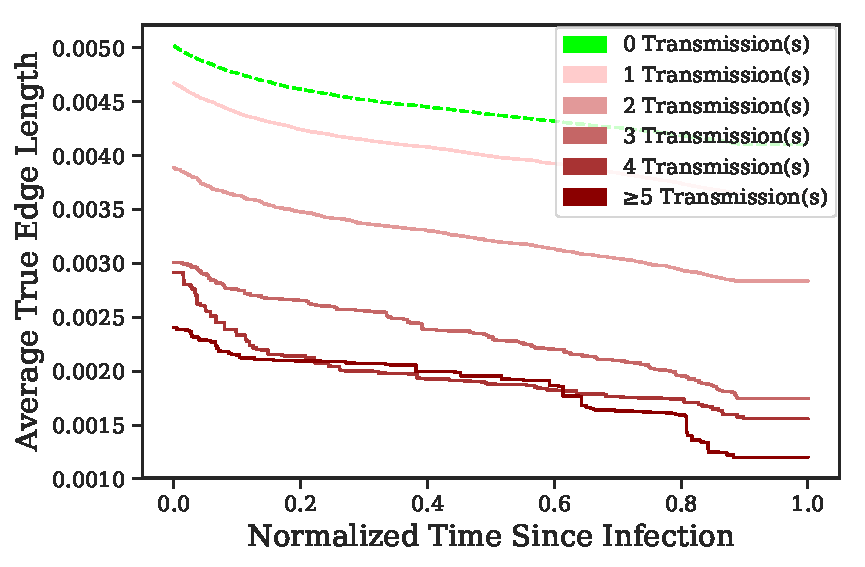
\includegraphics[width=0.65\textwidth]{figs/proact-true-bl-vs-time}
\caption[ProACT Diagram]
{As time progresses, the true incident branch length of each individual tends to decrease. This holds in inferred phylogenies as well (Fig.~\ref{fig:proact-diagram}d).}
\label{fig:proact-true-bl-vs-time}
\end{figure}

\begin{figure} % FIGURE S2 IN ORIGINAL PAPER
\centering
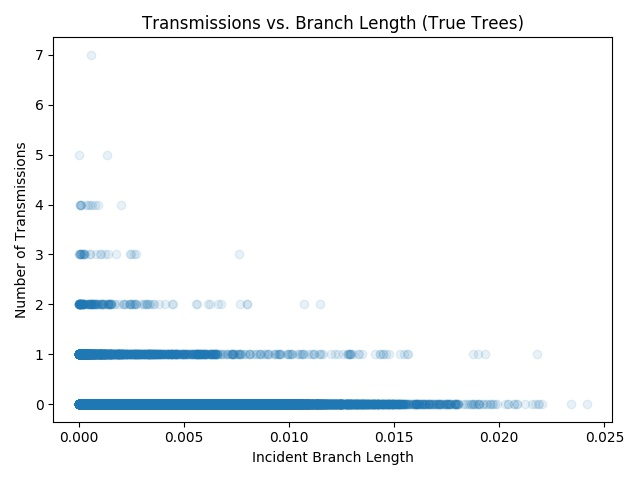
\includegraphics[width=0.495\textwidth]{figs/proact-trans-vs-bl-true}
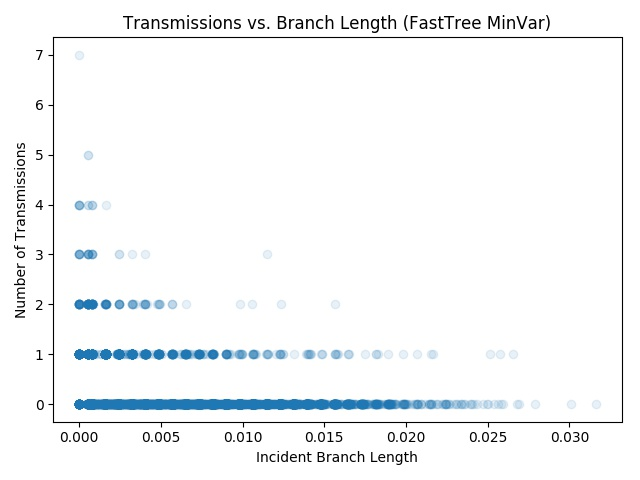
\includegraphics[width=0.495\textwidth]{figs/proact-trans-vs-bl-ftmv}
\caption[Number of Transmissions vs. Incident Branch Length]
{Number of transmissions vs. incident branch lengths for individuals in a simulated epidemic. The epidemic was run for 10 years, samples were obtained at the 9-year mark, and a phylogeny was inferred using FastTree~2 \cite{Price2010} and subsequently MinVar-rooted \cite{Mai2017}. Number of transmissions were measured between the 9-year and 10-year mark.}
\label{fig:proact-trans-vs-bl}
\end{figure}

\begin{figure} % FIGURE S3 IN ORIGINAL PAPER
\centering
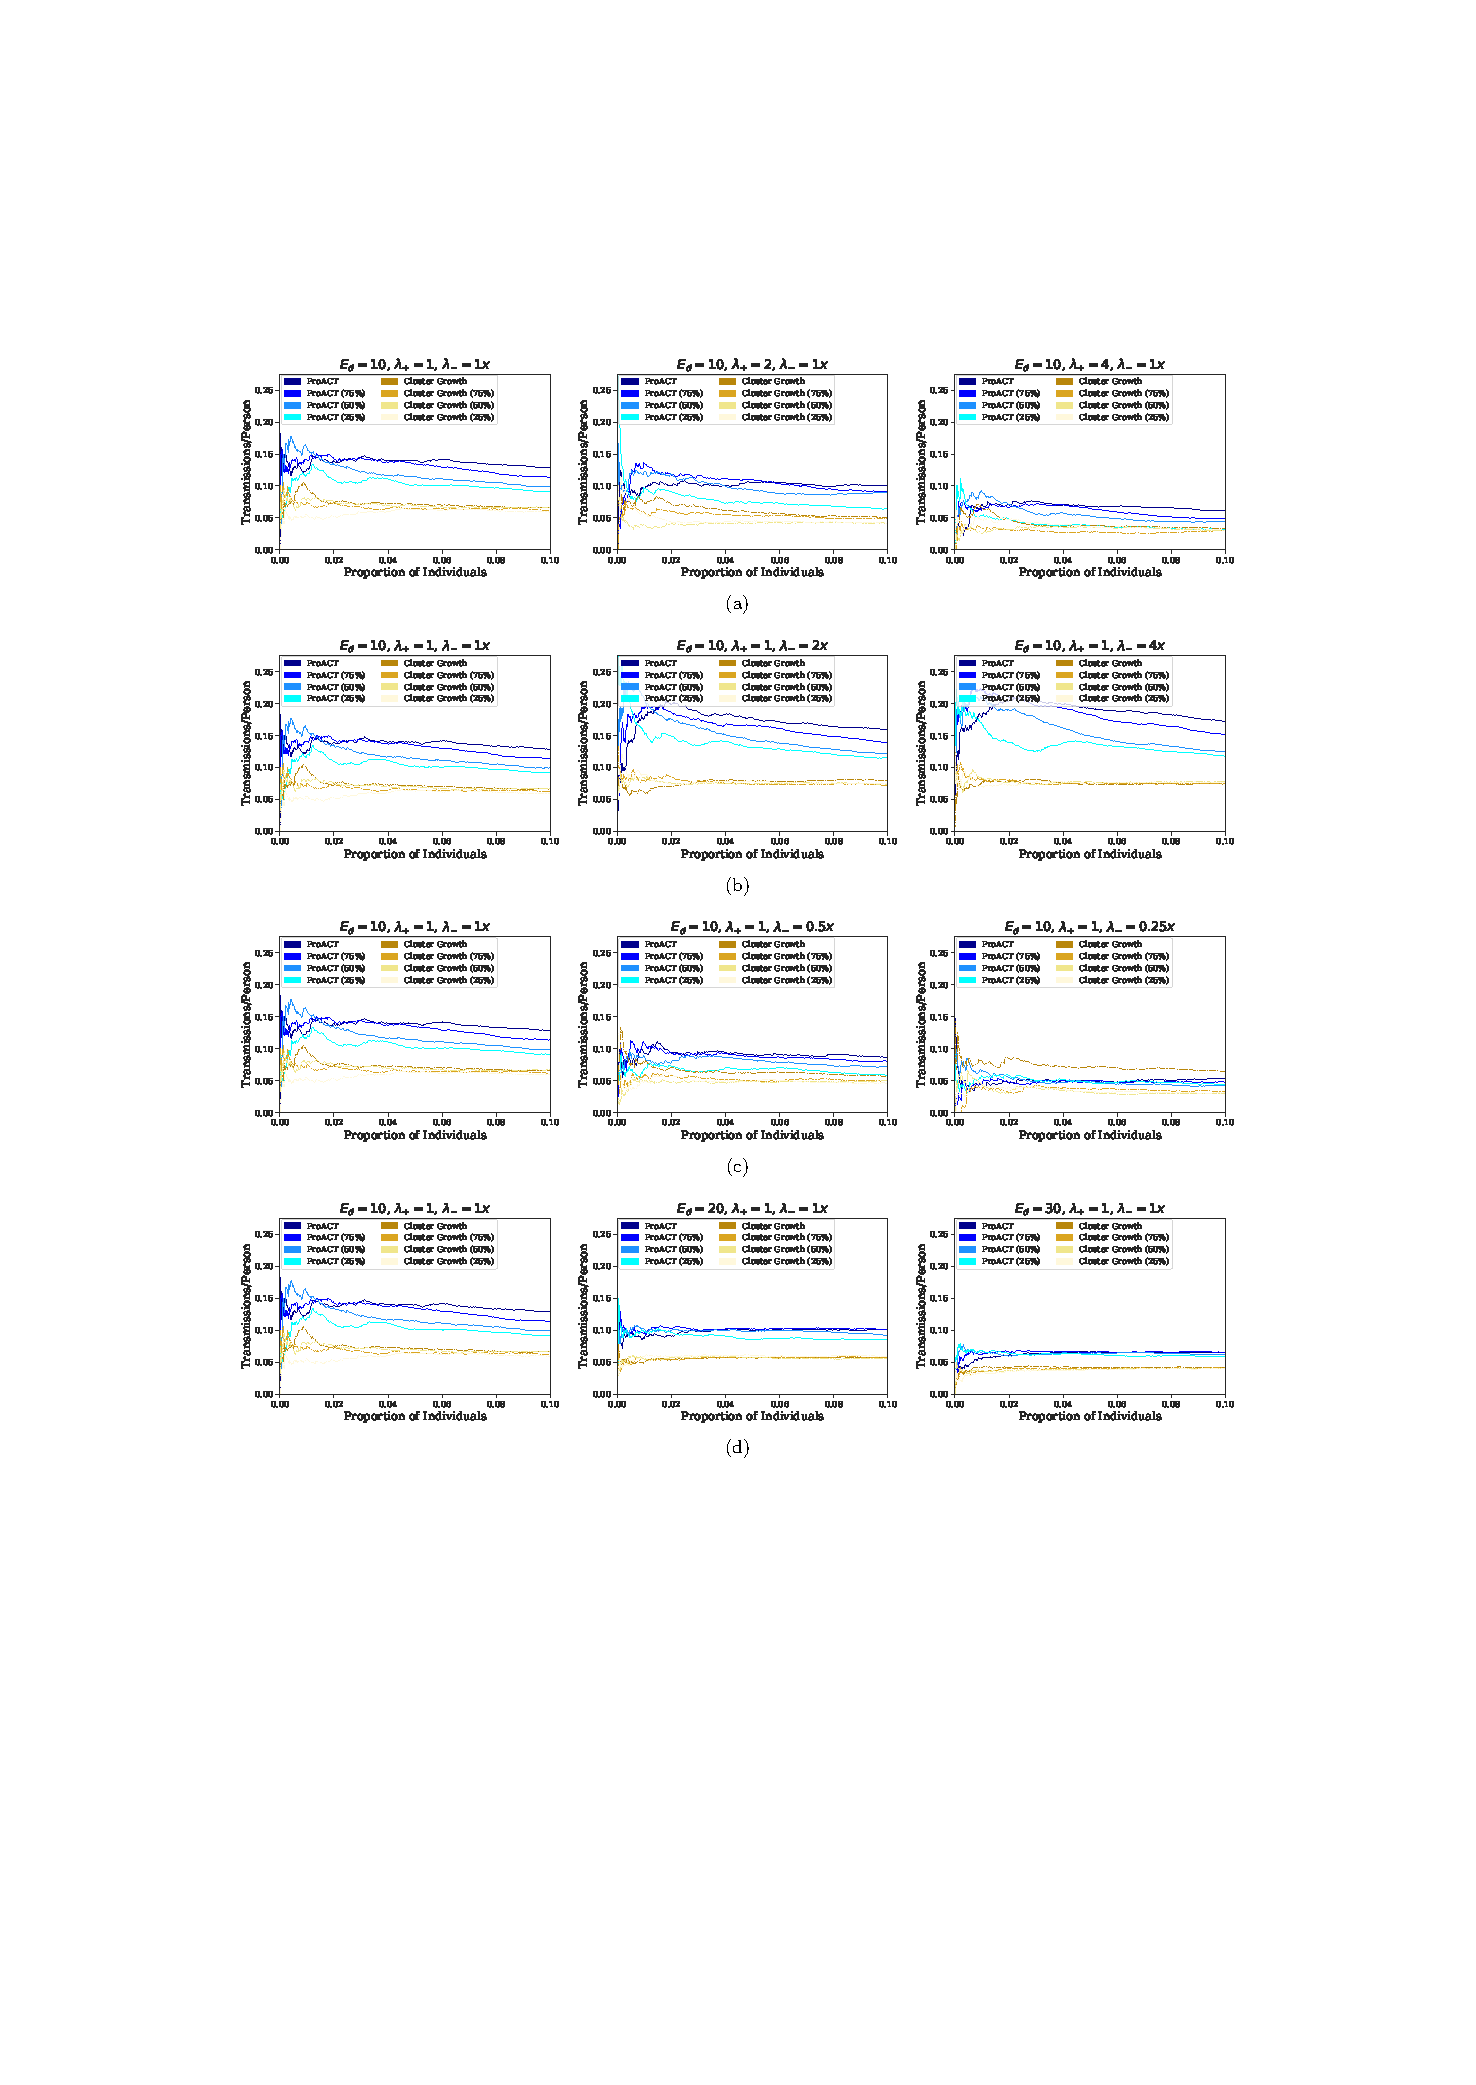
\includegraphics[width=0.85\textwidth]{figs/proact-efficacy-raw}
\caption[Raw ProACT Performance on Simulated Datasets]
{Efficacy on datasets simulated using FAVITES. \gls{CMA} of number of transmissions per person across all \glspl{PLWH} for each simulation parameter set.}
\label{fig:proact-efficacy-raw}
\end{figure}

\begin{figure} % FIGURE S4 IN ORIGINAL PAPER
\centering
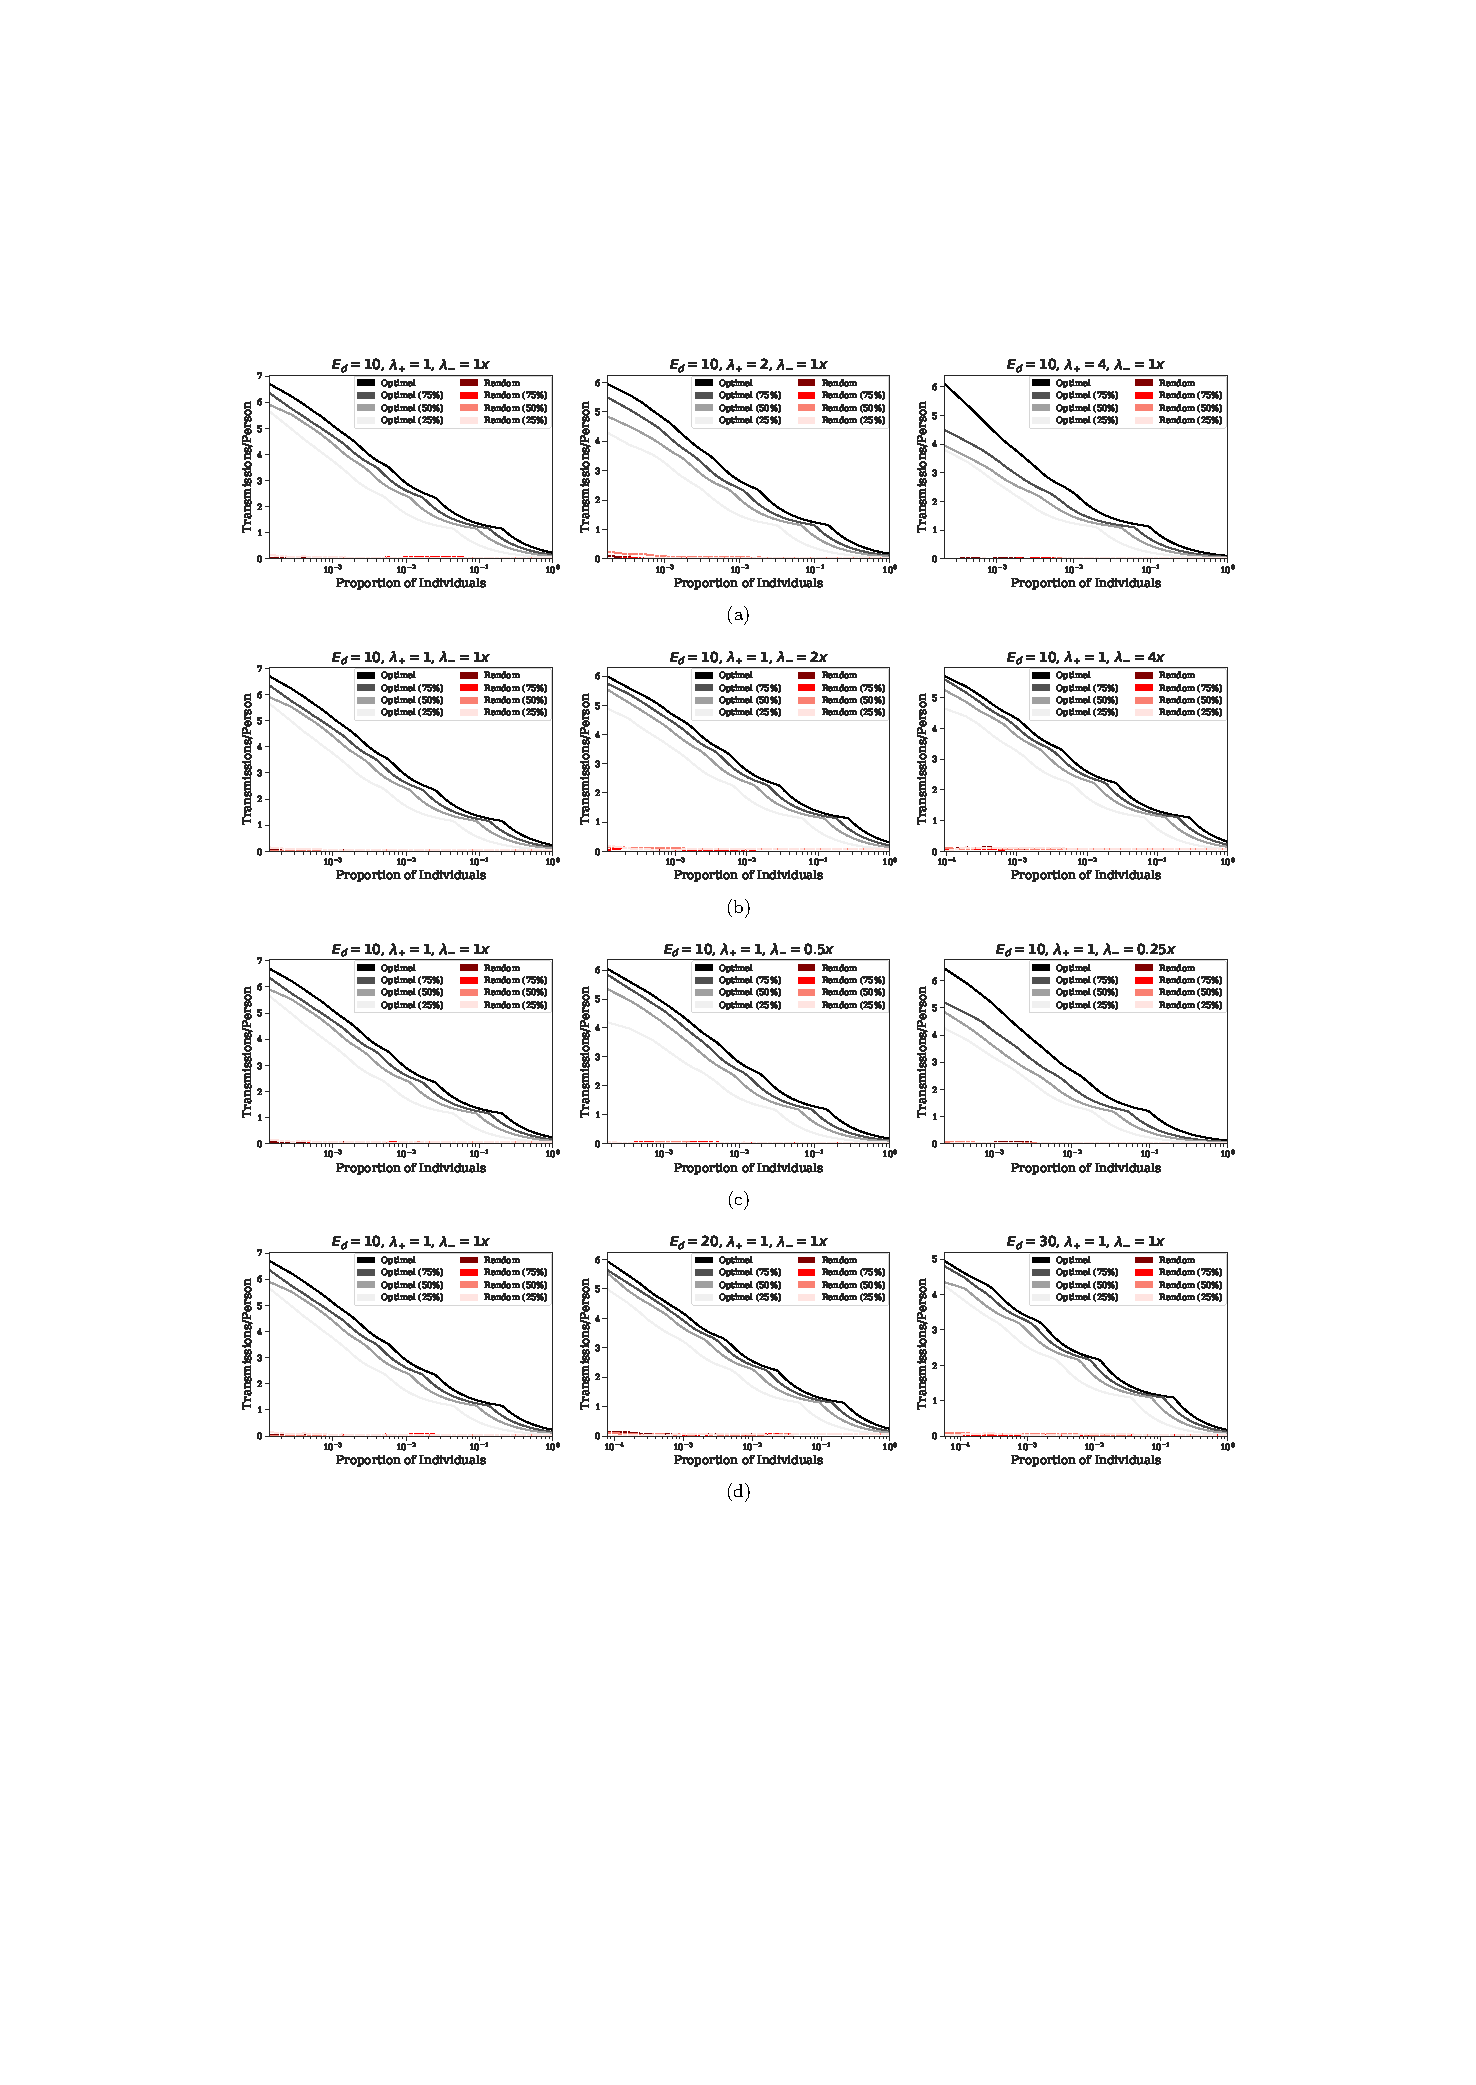
\includegraphics[width=0.85\textwidth]{figs/proact-efficacy-wide}
\caption[Optimal and Expected Raw Performance on Simulated Datasets]
{Efficacy of optimal and random selections on datasets simulated using FAVITES. \gls{CMA} of number of transmissions per person across all \glspl{PLWH} for each simulation parameter set.}
\label{fig:proact-efficacy-wide}
\end{figure}

\begin{figure} % FIGURE S5 IN ORIGINAL PAPER
\centering
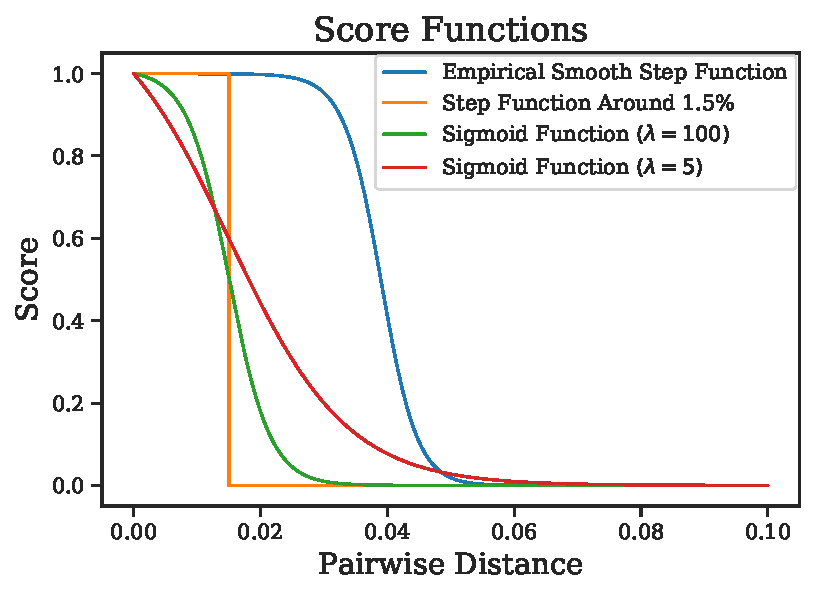
\includegraphics[width=0.65\textwidth]{figs/proact-scorefuncs}
\caption[Genetic Linkage Score Functions]
{Score functions vs. pairwise sequence distance.}
\label{fig:proact-scorefuncs}
\end{figure}

\begin{figure} % FIGURE S6 IN ORIGINAL PAPER
\centering
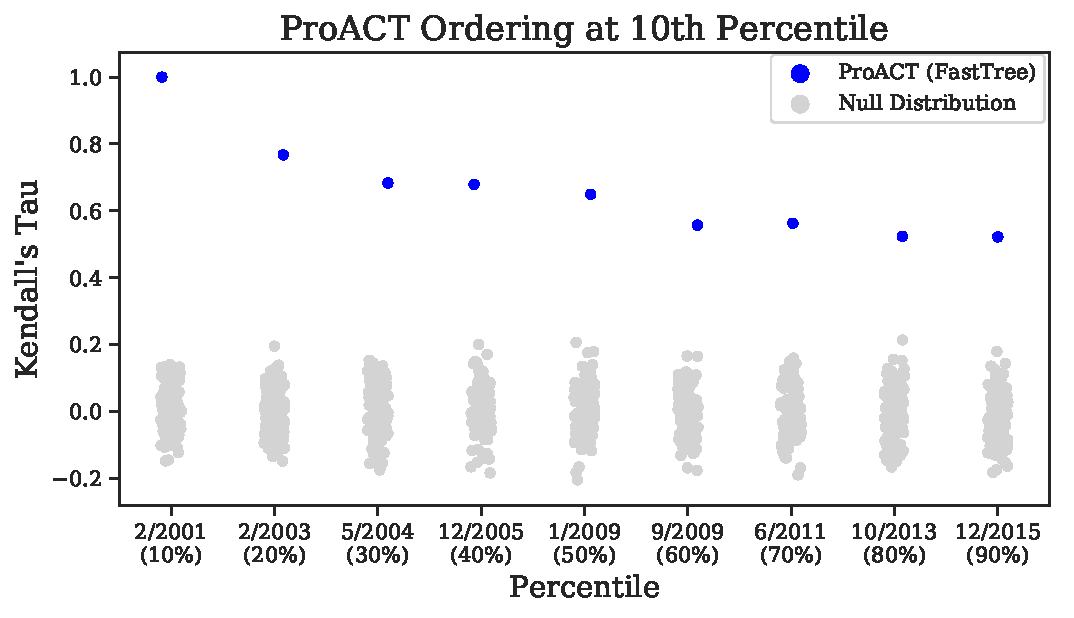
\includegraphics[width=0.85\textwidth]{figs/proact-tautest-first-proact}
\caption[Kendall's Tau-b Test vs. First ProACT Ordering]
{Kendall's tau-b test results for ProACT ordering with respect to the ProACT ordering obtained with only the first decile of the datasat. The full San Diego dataset was split into two sets (\textit{pre} and \textit{post}) at each decile (shown on the horizontal axis). The individuals in \textit{pre} were ordered using ProACT and by cluster growth. Kendall's tau-b correlation coefficient was computed for each ordering with respect to the ProACT ordering at the first decile. The null distribution was visualized by randomly shuffling the individuals in \textit{pre}.}
\label{fig:proact-tautest-first-proact}
\end{figure}

\begin{figure} % FIGURE S7 IN ORIGINAL PAPER
\centering
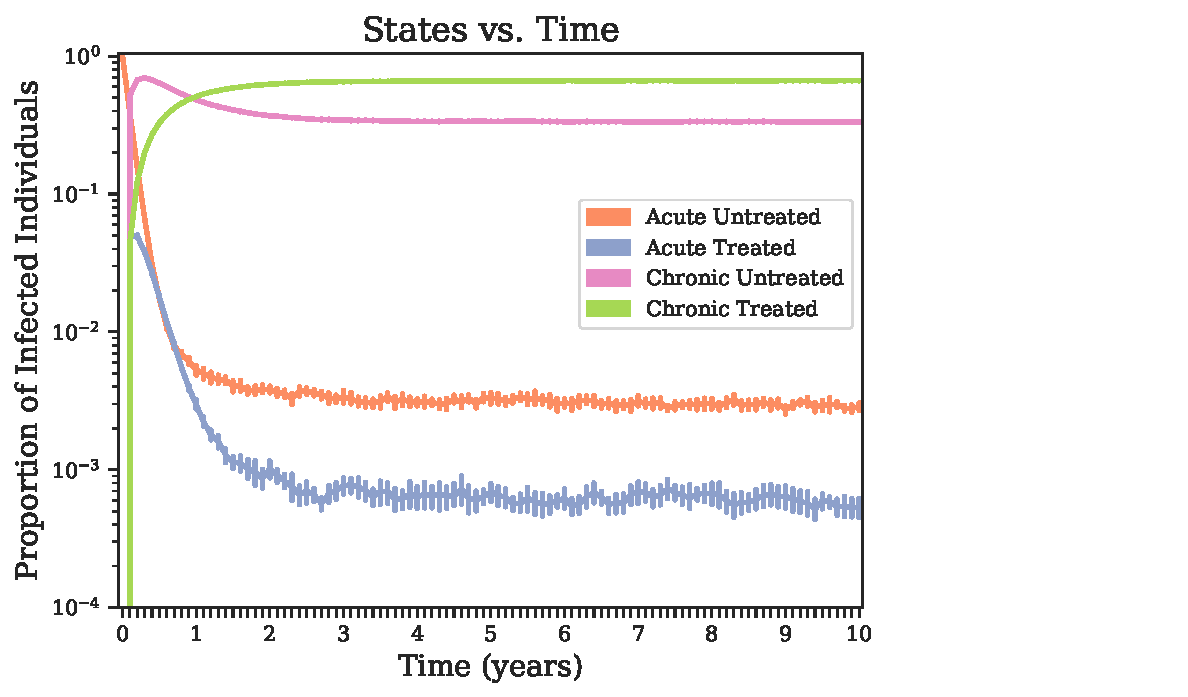
\includegraphics[width=0.65\textwidth]{figs/proact-prop-state-vs-time}
\caption[Proportion of Individuals in Infected States vs. Time]
{Proportion of individuals in each infected state (AU, AT, CU, and CT) vs. time in simulations in which all seed individuals at time 0 were placed in state AU.}
\label{fig:proact-prop-state-vs-time}
\end{figure}

%% END PROACT SUPPLEMENT